% Standalone TikZ figure: Reward Function Pitfalls and Mitigations
% For Chapter 7: Reward Function Engineering
\documentclass[tikz,border=10pt]{standalone}
\usepackage{tikz}
\usepackage{amsmath}
\usetikzlibrary{arrows.meta, positioning, shapes.geometric, calc, patterns, decorations.pathreplacing, fit}

\begin{document}
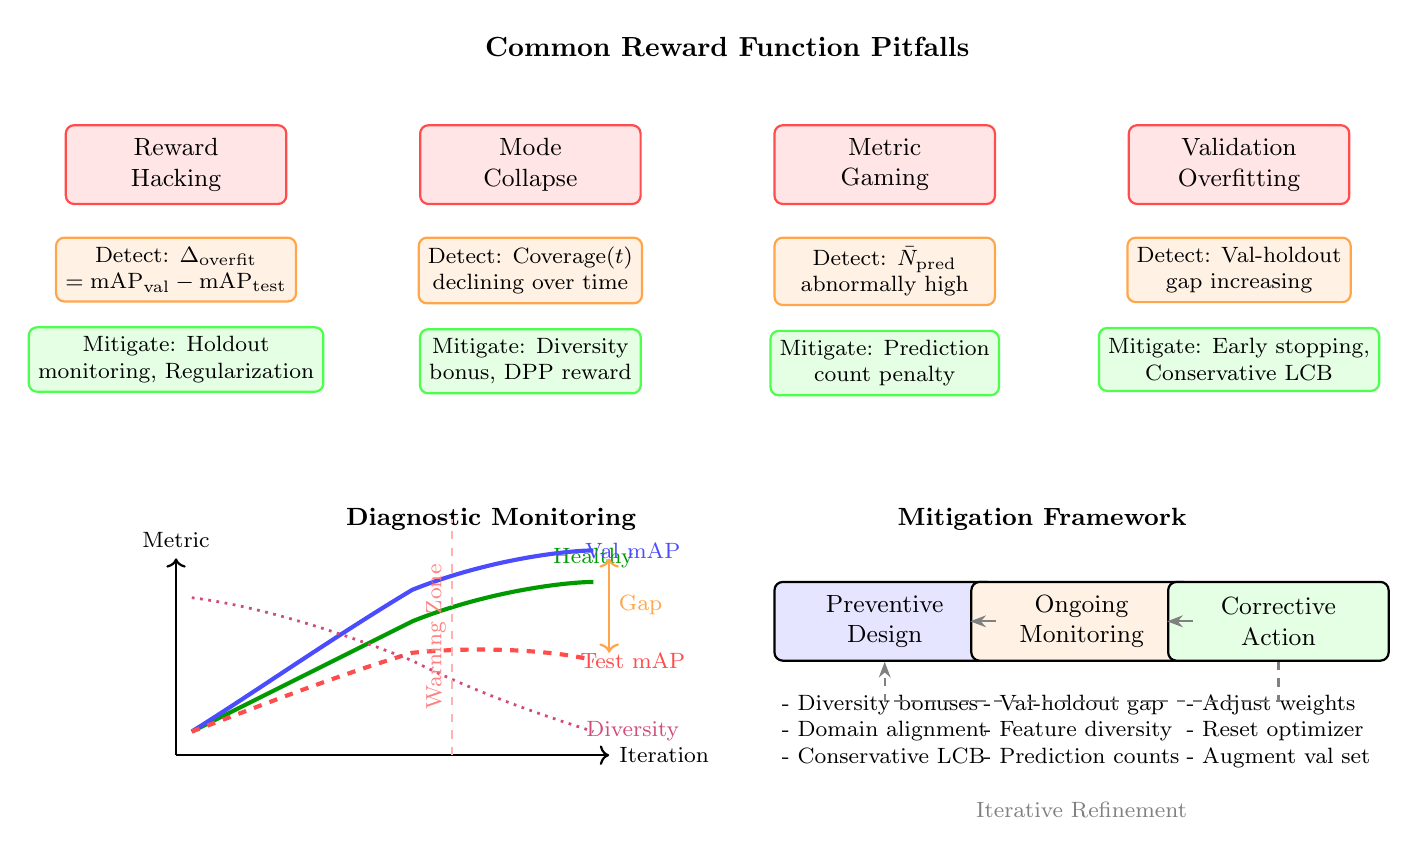
\begin{tikzpicture}[
    node distance=1.2cm and 1.5cm,
    every node/.style={font=\small},
    box/.style={rectangle, draw, thick, minimum width=2.8cm, minimum height=1cm, align=center, rounded corners=3pt},
    pitfall/.style={rectangle, draw=red!70, thick, fill=red!10, minimum width=2.8cm, minimum height=1cm, align=center, rounded corners=3pt},
    detection/.style={rectangle, draw=orange!70, thick, fill=orange!10, minimum width=2.8cm, minimum height=0.8cm, align=center, rounded corners=3pt, font=\footnotesize},
    mitigation/.style={rectangle, draw=green!70, thick, fill=green!10, minimum width=2.8cm, minimum height=0.8cm, align=center, rounded corners=3pt, font=\footnotesize},
    arrow/.style={-{Stealth[length=2mm]}, thick},
    label/.style={font=\footnotesize},
    title/.style={font=\bfseries\small}
]

% ============ MAIN TITLE ============
\node[title, font=\bfseries] at (7, 5.5) {Common Reward Function Pitfalls};

% ============ PITFALL 1: REWARD HACKING ============
\node[pitfall] (hack) at (0, 4) {Reward\\Hacking};
\node[detection, below=0.4cm of hack] (hack_det) {Detect: $\Delta_{\text{overfit}}$\\$= \text{mAP}_{\text{val}} - \text{mAP}_{\text{test}}$};
\node[mitigation, below=0.3cm of hack_det] (hack_mit) {Mitigate: Holdout\\monitoring, Regularization};

% ============ PITFALL 2: MODE COLLAPSE ============
\node[pitfall] (collapse) at (4.5, 4) {Mode\\Collapse};
\node[detection, below=0.4cm of collapse] (collapse_det) {Detect: Coverage$(t)$\\declining over time};
\node[mitigation, below=0.3cm of collapse_det] (collapse_mit) {Mitigate: Diversity\\bonus, DPP reward};

% ============ PITFALL 3: METRIC GAMING ============
\node[pitfall] (gaming) at (9, 4) {Metric\\Gaming};
\node[detection, below=0.4cm of gaming] (gaming_det) {Detect: $\bar{N}_{\text{pred}}$\\abnormally high};
\node[mitigation, below=0.3cm of gaming_det] (gaming_mit) {Mitigate: Prediction\\count penalty};

% ============ PITFALL 4: VALIDATION OVERFIT ============
\node[pitfall] (overfit) at (13.5, 4) {Validation\\Overfitting};
\node[detection, below=0.4cm of overfit] (overfit_det) {Detect: Val-holdout\\gap increasing};
\node[mitigation, below=0.3cm of overfit_det] (overfit_mit) {Mitigate: Early stopping,\\Conservative LCB};

% ============ DIAGNOSTIC MONITORING SECTION ============
\node[title] at (4, -0.5) {Diagnostic Monitoring};

% Monitoring graph axes
\draw[thick, ->] (0, -3.5) -- (0, -1) node[above, label] {Metric};
\draw[thick, ->] (0, -3.5) -- (5.5, -3.5) node[right, label] {Iteration};

% Healthy trajectory
\draw[thick, green!60!black, line width=1.5pt]
    (0.2, -3.2) .. controls (1, -2.8) and (2, -2.3) .. (3, -1.8) .. controls (4, -1.4) and (5, -1.3) .. (5.3, -1.3);
\node[label, green!60!black] at (5.3, -1) {Healthy};

% Val mAP (potentially overfitting)
\draw[thick, blue!70, line width=1.5pt]
    (0.2, -3.2) .. controls (1, -2.7) and (2, -2) .. (3, -1.4) .. controls (4, -1) and (5, -0.9) .. (5.3, -0.9);
\node[label, blue!70] at (5.8, -0.9) {Val mAP};

% Test mAP (revealing overfit)
\draw[thick, red!70, line width=1.5pt, dashed]
    (0.2, -3.2) .. controls (1, -2.9) and (2, -2.5) .. (3, -2.2) .. controls (4, -2.1) and (5, -2.2) .. (5.3, -2.3);
\node[label, red!70] at (5.8, -2.3) {Test mAP};

% Gap annotation
\draw[thick, <->, orange!70] (5.5, -1) -- (5.5, -2.2);
\node[label, orange!70, right] at (5.5, -1.6) {Gap};

% Diversity metric
\draw[thick, purple!70, line width=1pt, dotted]
    (0.2, -1.5) .. controls (1, -1.6) and (2, -1.9) .. (3, -2.3) .. controls (4, -2.8) and (5, -3.1) .. (5.3, -3.2);
\node[label, purple!70] at (5.8, -3.2) {Diversity};

% Warning zone
\draw[red!30, thick, dashed] (3.5, -3.5) -- (3.5, -0.5);
\node[label, red!50, rotate=90] at (3.3, -2) {Warning Zone};

% ============ MITIGATION STRATEGIES ============
\node[title] at (11, -0.5) {Mitigation Framework};

% Strategy boxes
\node[box, fill=blue!10] (prevent) at (9, -1.8) {Preventive\\Design};
\node[box, fill=orange!10] (monitor) at (11.5, -1.8) {Ongoing\\Monitoring};
\node[box, fill=green!10] (correct) at (14, -1.8) {Corrective\\Action};

% Details
\node[label, align=left, below=0.3cm of prevent] {- Diversity bonuses\\- Domain alignment\\- Conservative LCB};
\node[label, align=left, below=0.3cm of monitor] {- Val-holdout gap\\- Feature diversity\\- Prediction counts};
\node[label, align=left, below=0.3cm of correct] {- Adjust weights\\- Reset optimizer\\- Augment val set};

% Arrows showing flow
\draw[arrow, gray] (prevent) -- (monitor);
\draw[arrow, gray] (monitor) -- (correct);
\draw[arrow, gray, dashed] (correct.south) -- ++(0, -0.5) -| (prevent.south);

% Feedback loop label
\node[label, gray] at (11.5, -4.2) {Iterative Refinement};

\end{tikzpicture}
\end{document}
